\documentclass[journal]{IEEEtran}

\usepackage{amsmath,amssymb}
\usepackage{array}
\usepackage{booktabs}
\usepackage{balance}
\usepackage{graphicx}
\usepackage{tabularx}
\usepackage{url}

\newcommand{\ours}{FedTwin-CryptID}
\newcommand{\vectheta}{\boldsymbol{\theta}}

\begin{document}

\title{Supplementary Material for ``\ours: Federated Fixed-Evidence Calibration and Audit for Multimedia Copy Review''}
\author{Chandrasen~Pandey}
\maketitle

\section{Feature and Optimization Details}

The evaluated system consumes fixed query--reference evidence and never exports raw media or raw embeddings. The linear schema contains visual, audio, and temporal similarity; modality reliability; agreement/gap terms; frame-ratio and transformation context; reliability-weighted scores; maximum, mean, and product fusion; and optional category/client fields. The default invariant policy excludes direct category, genre, and client indicators. For selected roots $x_j$, the polynomial map appends $x_j^2$ and $x_jx_l$ and is standardized using training-split statistics only.

For client $k$, binary cross-entropy with $L_2$ regularization is
\begin{equation}
L_k(\vectheta)=-\frac{1}{n_k}\sum_i y_i\log p_i+(1-y_i)\log(1-p_i)+\lambda\lVert\vectheta\rVert_2^2.
\end{equation}
FedAvg computes $\vectheta_{t+1}=\vectheta_t+\sum_k(n_k/n)\Delta_k$. FedProx adds $\mu\lVert\vectheta-\vectheta_t\rVert_2^2/2$ to each local objective. The reported compact-head settings use $\lambda=10^{-4}$, $\mu=0.02$, and the seeds/configuration frozen in \texttt{configs/paper.yaml}. Personalized heads initialize from the final global head and fit only client-local calibration rows.

\begin{table}[!t]
\centering
\caption{Feature-policy roles.}
\scriptsize
\begin{tabularx}{\columnwidth}{p{0.25\columnwidth}p{0.28\columnwidth}X}
\toprule
Family & Examples & Default role \\
\midrule
Scores & visual, audio, temporal & Included \\
Reliability & visual/audio reliability, weighted scores & Included \\
Agreement & gap, mean, max, product & Included \\
Transform & frame ratio, scenario indicator & Audit dependent \\
Context & category, genre, client/domain & Excluded; leakage audit only \\
\bottomrule
\end{tabularx}
\end{table}

\section{Frozen Splits and Statistical Procedure}

For every confirmatory VCSL and FMA tier, positive-pair connected components are indivisible split units. Components are assigned deterministically from the seed; negatives are sampled only from assets assigned to that split. The verifier rejects null IDs, self-pairs, duplicate directional pairs, nonbinary labels, and any train/test asset intersection. Released manifests record positive, negative, pair, asset, query, client, and decode counts. Restricted descriptors and media are not redistributed.

Metrics are computed on fixed held-out rows. We report PR-AUC, ROC-AUC, FPR at 95\% recall, Brier score, 15-bin expected calibration error, Recall@$K$, mAP, fixed-budget recall, and workload. Query-ranking confidence intervals resample query clusters with replacement. Method deltas use paired bootstrap and paired sign-flip permutation tests on the same examples. Holm's step-down procedure adjusts the family of method-comparison $p$-values. Effect sizes and 95\% intervals accompany adjusted significance values; a $p$-value alone is not treated as evidence of practical improvement. The hardest 1:10000 stress has 100 positive-bearing queries and 1,000,100 candidate instances per seed. Because the public label topology has fewer than 10,001 unique references, it repeats reference assets with independent noise realizations and is not a 10,000-unique-reference benchmark.

At prevalence $\pi$, measured recall $r$, and false-positive rate $f$, expected review precision is
\begin{equation}
\operatorname{Prec}(\pi)=\frac{\pi r}{\pi r+(1-\pi)f},
\end{equation}
and expected reviews per true positive are $1/\operatorname{Prec}(\pi)$. These are prevalence projections, not new detector measurements.

\section{Communication-Round Ablation}

The clean VCSL public-label confirmatory run records each of 20 communication
rounds for seeds 31, 37, and 41. Fig.~\ref{fig:round-ablation} reports the mean
client training loss for plain FedAvg, FedProx, SecureAgg-simulation FedAvg,
and quantized-proxy FedAvg. All four traces use the same frozen split and local
epoch count. The protected modes follow plain FedAvg to plotting precision,
while most optimization progress occurs in the early rounds. This is a
convergence audit, not an independent held-out-utility gain claim.

\begin{figure}[!t]
  \centering
  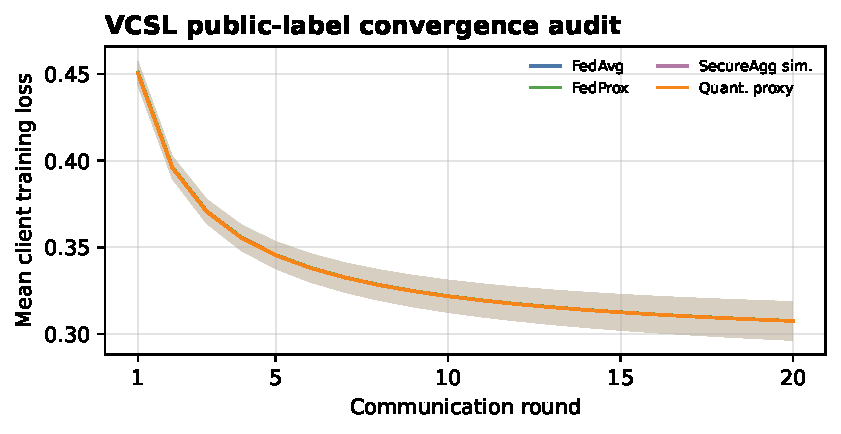
\includegraphics[width=0.96\columnwidth]{figures/communication_round_ablation.pdf}
  \caption{Three-seed communication-round ablation on the confirmatory VCSL
  public-label tier. Lines are mean client training loss; bands are sample
  standard deviation across seeds.}
  \label{fig:round-ablation}
\end{figure}

\section{Protected Aggregation Semantics}

The implementation exposes four accurately named modes. Plain FedAvg/FedProx sends floating-point compact updates. \texttt{secureagg\_sim} applies deterministic pairwise masks whose signed contributions cancel in the active-client sum; 0\%, 10\%, and 20\% post-mask dropout scenarios reconstruct and remove residual masks and check active-weight renormalization. It does not implement authenticated key agreement, secret sharing, collusion resistance, or production recovery. \texttt{quantized\_transport\_proxy} quantizes/dequantizes updates and reports error, safe range, and byte accounting; it is not homomorphic encryption.

The Paillier mode uses 2048-bit keys for the three reported measurements (seeds 31, 37, and 41). For scale $S$, client weight integer $w_k$, and clipped quantized coordinate $m_{kj}=\operatorname{round}(S\Delta_{kj})$, the server multiplies Paillier ciphertexts to obtain an encryption of $\sum_kw_km_{kj}$. Only the aggregate is decrypted and divided by $S\sum_kw_k$. The artifact reports per-seed key size, quantization scale and safe range, maximum absolute error, encryption time, aggregate/decryption time, plaintext and ciphertext bytes, and expansion. Fast tests may use smaller keys and are explicitly excluded from paper evidence.

\begin{table}[!t]
\centering
\caption{Protection claims and exclusions.}
\scriptsize
\begin{tabularx}{\columnwidth}{p{0.25\columnwidth}p{0.29\columnwidth}X}
\toprule
Mode & Demonstrated & Not demonstrated \\
\midrule
Plain & Optimization reference & Update confidentiality \\
SecureAgg simulation & Mask cancellation/dropout behavior & Production security proof \\
Quantized proxy & Numeric/transport effects & Encryption \\
Paillier & Additive compact-update sum & Threshold keys or encrypted media inference \\
\bottomrule
\end{tabularx}
\end{table}

\balance
\section{Receipt Semantics and Threat Boundary}

A receipt contains salted media commitments, model/configuration/evidence digests, a monotone sequence or timestamp, the previous-receipt hash, the signer public key, and an Ed25519 signature. Canonical serialization is hashed before signing. Verification recomputes all commitments, checks the signature, and verifies chain linkage. Tamper tests alter payload and predecessor fields independently.

Receipts establish consistency, ordering, and signer accountability under the active key. They do not establish that the detector is correct, that a claimant owns media, that feature extraction was honest, or that legal infringement occurred. The honest-but-curious aggregation scope keeps raw media and embeddings local but does not provide differential privacy or complete protection against update inference. Poisoning experiments are controlled compact-head stress tests, not a proof against adaptive Byzantine clients.

\section{Artifact Map and Reproduction}

The release contains strict configuration, run/result manifests, claim mappings, permitted CSV/JSON results, table sources, finite figure sources, checksums, and expected outputs. Raw copyrighted media, downloaded descriptors, caches, bytecode, temporary files, and private paths are excluded. Confirmatory VCSL and FMA rows map to clean-commit run manifests and complete selected-input/output records; any retained historical row is explicitly marked exploratory and is not used for a confirmatory claim.

The four entry points are \texttt{fedtwin smoke}, \texttt{fedtwin reproduce}, \texttt{fedtwin regenerate-paper}, and \texttt{fedtwin verify-artifact}. Complete copyable commands and the table/figure map are in \texttt{docs/REPRODUCIBILITY.md}.

Each run records the Git commit, canonical configuration hash, seed, dependency versions, input/output hashes, row/client counts, feature schema, timing, Python/platform, and hardware. The same seed/configuration must reproduce scientific JSON/CSV fields exactly; wall-clock time and latency fields are runtime provenance and may vary. Regenerated paper metrics are checked to $10^{-4}$. The repository URL is \url{https://github.com/Devchandrasen/fedtwin-cryptid}. The archival DOI will be added only after the verified GitHub release is deposited.

\section{Additional Limitations}

VCSL visual and FMA audio tiers are separate; the synthetic conflict tier does not establish synchronized audiovisual fusion. Public-label topology features are not raw-descriptor localization. The work does not claim state-of-the-art copy retrieval, formal differential privacy, production SecureAgg, encrypted inference, ownership adjudication, or automatic enforcement. Dataset licenses remain with upstream providers. Human review, ownership validation, appeals, and receipt supersession are required before action on a flagged candidate.

\end{document}
